
\documentclass[paper=letter, fontsize=11pt]{scrartcl} % A4 paper and 11pt font size

\usepackage[T1]{fontenc} % Use 8-bit encoding that has 256 glyphs
\usepackage{fourier} % Use the Adobe Utopia font for the document - comment this line to return to the LaTeX default
\usepackage[english]{babel} % English language/hyphenation
\usepackage{amsmath,amsfonts,amsthm} % Math packages
\usepackage{bm}
\usepackage{graphicx}
\usepackage[section]{placeins}

\usepackage{sectsty} % Allows customizing section commands
\allsectionsfont{\centering \normalfont\scshape} % Make all sections centered, the default font and small caps

\usepackage{fancyhdr} % Custom headers and footers
\pagestyle{fancyplain} % Makes all pages in the document conform to the custom headers and footers
\fancyhead{} % No page header - if you want one, create it in the same way as the footers below
\fancyfoot[L]{} % Empty left footer
\fancyfoot[C]{} % Empty center footer
\fancyfoot[R]{\thepage} % Page numbering for right footer
\renewcommand{\headrulewidth}{0pt} % Remove header underlines
\renewcommand{\footrulewidth}{0pt} % Remove footer underlines
\setlength{\headheight}{13.6pt} % Customize the height of the header

\numberwithin{equation}{section} % Number equations within sections (i.e. 1.1, 1.2, 2.1, 2.2 instead of 1, 2, 3, 4)
\numberwithin{figure}{section} % Number figures within sections (i.e. 1.1, 1.2, 2.1, 2.2 instead of 1, 2, 3, 4)
\numberwithin{table}{section} % Number tables within sections (i.e. 1.1, 1.2, 2.1, 2.2 instead of 1, 2, 3, 4)

\setlength\parindent{0pt} % Removes all indentation from paragraphs - comment this line for an assignment with lots of text

%----------------------------------------------------------------------------------------
%   TITLE SECTION
%----------------------------------------------------------------------------------------

\newcommand{\horrule}[1]{\rule{\linewidth}{#1}} % Create horizontal rule command with 1 argument of height

\title{ 
\normalfont \normalsize 
\textsc{Steward Observatory} \\ [25pt] % Your university, school and/or department name(s)
\horrule{0.5pt} \\[0.4cm] % Thin top horizontal rule
\huge Direct Imaging Assignment \\ % The assignment title
\horrule{2pt} \\[0.5cm] % Thick bottom horizontal rule
}

\author{Yifan Zhou} % Your name

\date{\normalsize\today} % Today's date or a custom date

\begin{document}

\maketitle % Print the title
\section{Median Combined Image}
\begin{figure}[!h]
  \centering
  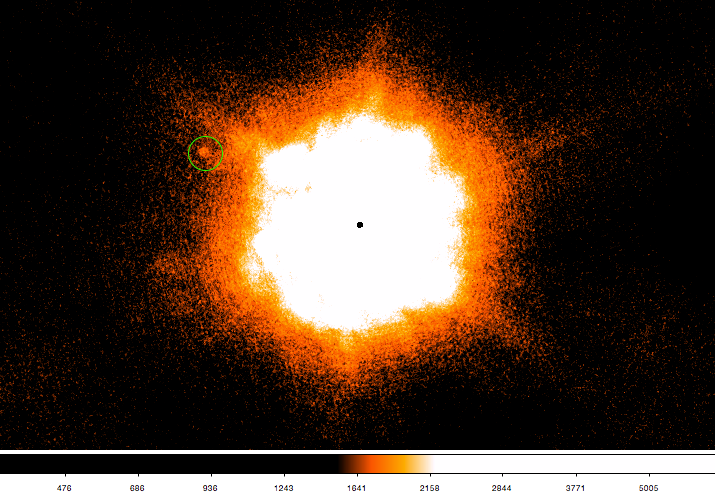
\includegraphics[width=\textwidth]{median}
  \caption{Median Combined Image for HR8799 system. On this image,
    only HR8799 b is clearly shown.}
  \label{fig:median}
\end{figure}
\subsection{Contrast Curve}
The procedure to make the contrast curve is described as following.
\begin{enumerate}
\item Add unsaturated PSFs  into original un-rotated images as fake
  planets. Fake planets are evenly placed 0 to 3 arcsec away from the
  peak of the primary star. A median combination of images with fake
  planets is presented in Figure \ref{fig:median_fakeplanet}. The peak
  value of the fake planet is fixed, and defined as
  $\mathrm{Amp_{PSF}}$
  
   \begin{figure}
    \centering
    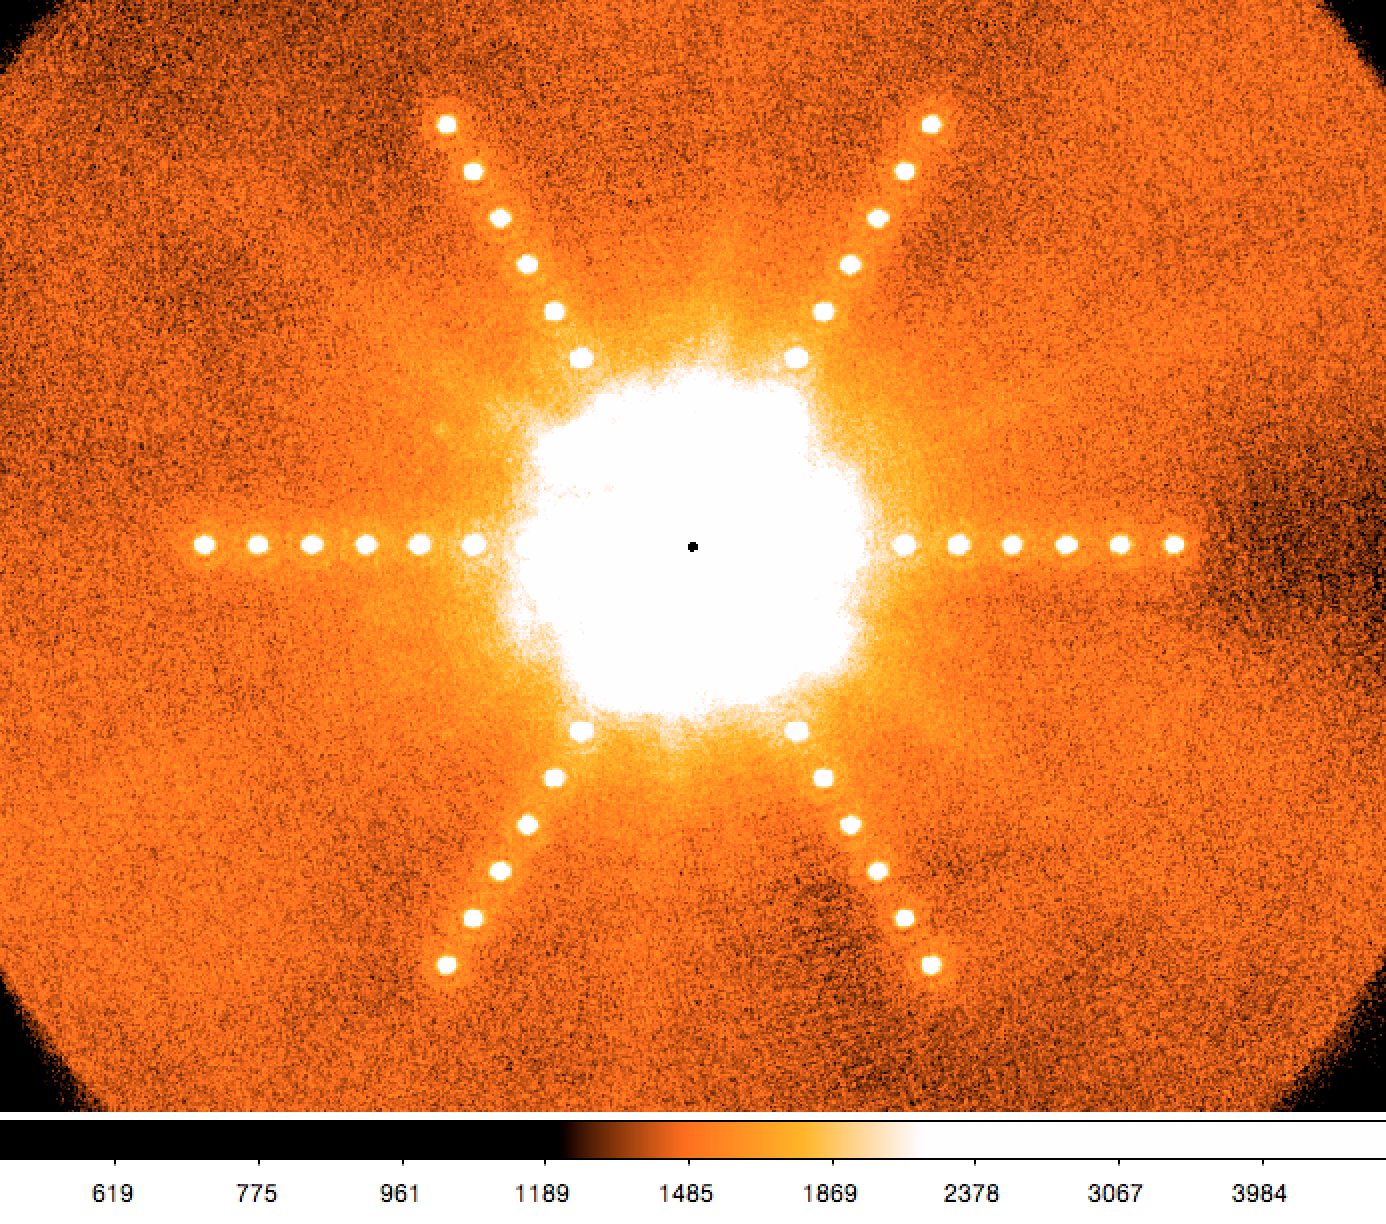
\includegraphics[width=\textwidth]{median_fake}
    \caption{Median combination of images with fake planets adding
      in. }
    \label{fig:median_fakeplanet}
  \end{figure}
 \item Noise is measured in an annulus around the  fake planet. The
   inner and outer radii of the annulus are 15 and 20 pixels. I define
   the noise as the square root of the second moment of the pixel
   values in the annulus to avoid negative value due to Primary
   subtraction.
   \[
     \mathrm{Noise} = \sqrt{\frac{1}{n}\sum_{i=1}^{n}F_{n}^{2}}
     \]
 \item S/N is defined as peak value of PSF   $\mathrm{Amp_{PSF}}$ and
   the Noise calculated as above. Contrast curve is defined as the
   relationship of S/N and angular separation. Figure
   \ref{fig:median_curve} presents the contrast curve for median
   combined image with   $\mathrm{Amp_{PSF}} = 2000$.
 \end{enumerate}

 \begin{figure}
   \centering
   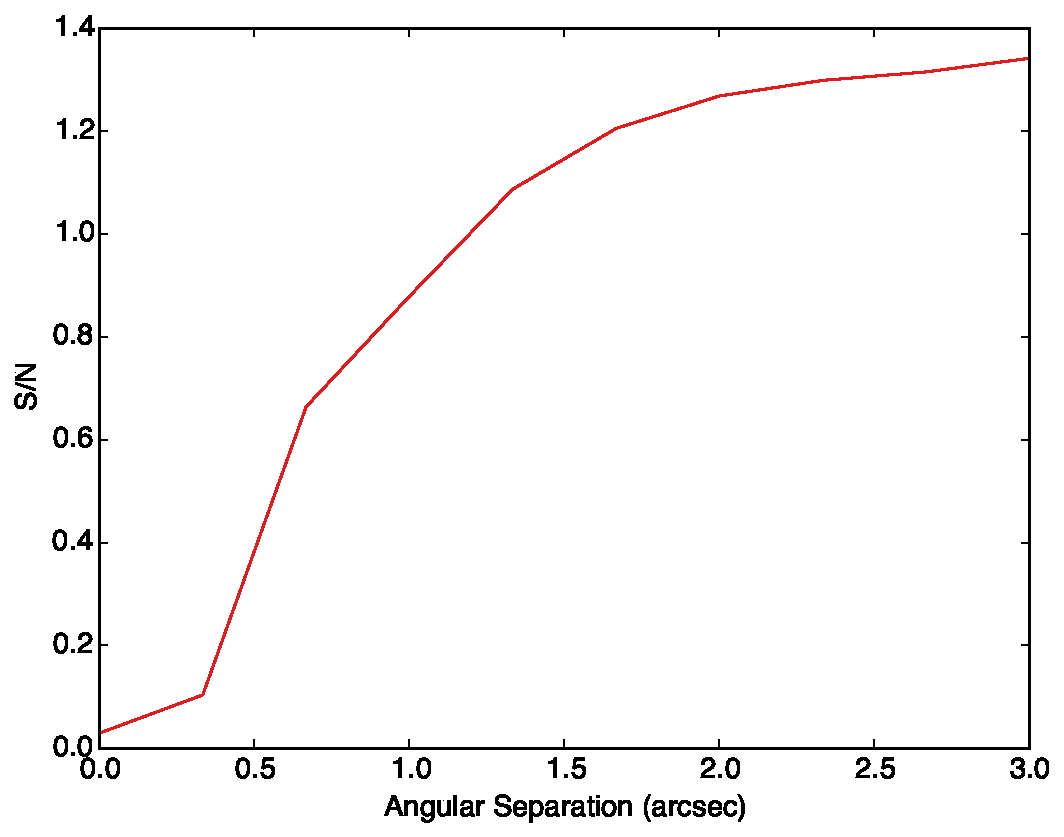
\includegraphics[width=\textwidth]{median_contrastCurve_amp=2000}
   \caption{Contrast curve for meian combined image. The PSF that used
     as fake planet is scaled so that the peak value is equal to
     2000. }
   \label{fig:median_curve}
 \end{figure}
 
 \section{ADI}
 \section{Simple ADI}
 ADI method applied here is the simplest case that illustrate in
 Marois et. al. (2008). Every image except the target image is treated
 as PSF image. The PSF is constructed by the median combining of all
 PSF images. No selection of PSF images or calculation of any scale
 factors is carried out here. The result of simple ADI application is
 shown in Figure \ref{fig:simple_adi}.

ADI processed image with fake planets injected is shown in Figure
\ref{fig:adi_fakeplanet}. In the image, it is clearly shown that self
subtraction is very severe. This is due to coarse selection of PSF
images. In a more sophisticated manner, the PSF images should be
selected with angular distances that are above certain threshold
compare to the target image to avoid self subtraction.

S/N curve is shown in Figure \ref{fig:adi_median_curve}. In general,
ADI improves  signal to noise significantly. However, odd shape of the
curve appears at around $2.5''$. I think this is also caused by self
subtraction.

\begin{figure}[!h]
  \centering
  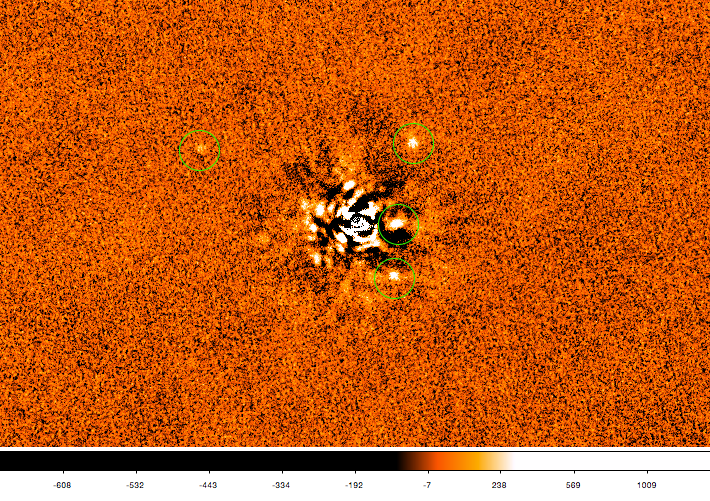
\includegraphics[width=\textwidth]{simple_ADI}
  \caption{HR8799 primary star subtracted with ADI technique. HR8799b,
    c, d now are clearly shown on the image. The bright spot near
    HR8799e is hardly tell whether it is the image of HR8799e or it is
    a quasi bright speckle.}
  \label{fig:simple_adi}
\end{figure}

   \begin{figure}
    \centering
    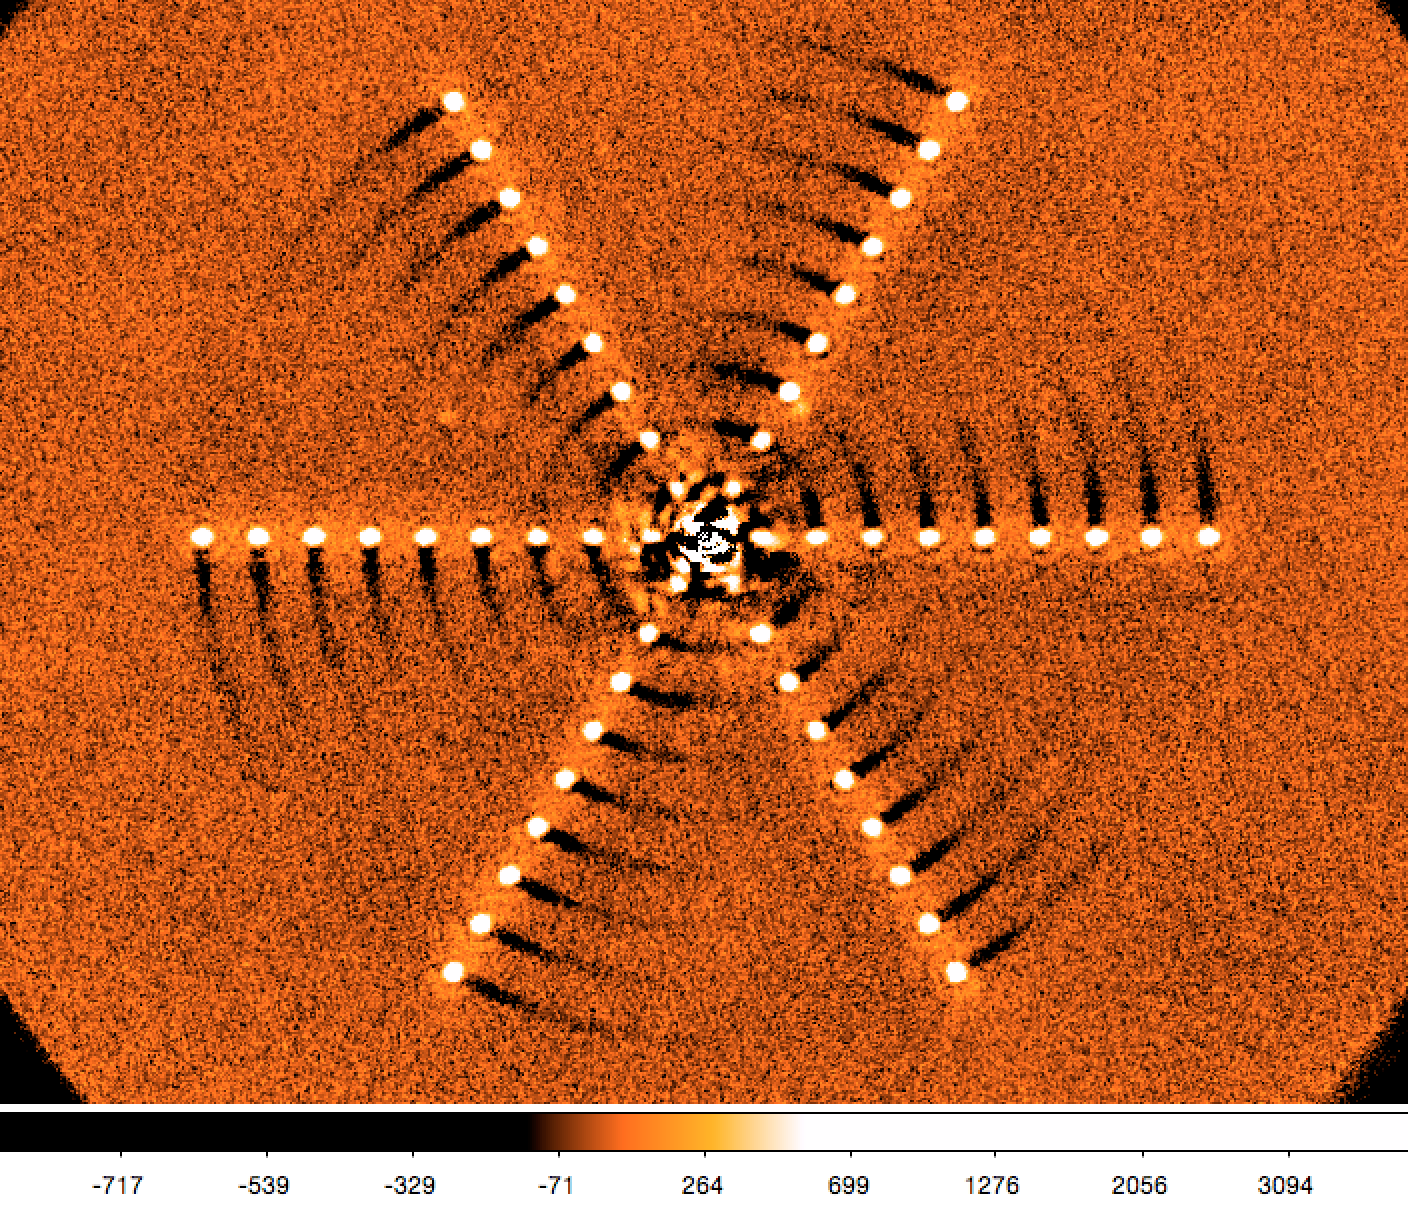
\includegraphics[width=\textwidth]{adi_fake}
    \caption{Image with primary subtracted using ADI with fake planets adding
      in.}
    \label{fig:adi_fakeplanet}
  \end{figure}

  \begin{figure}
   \centering
   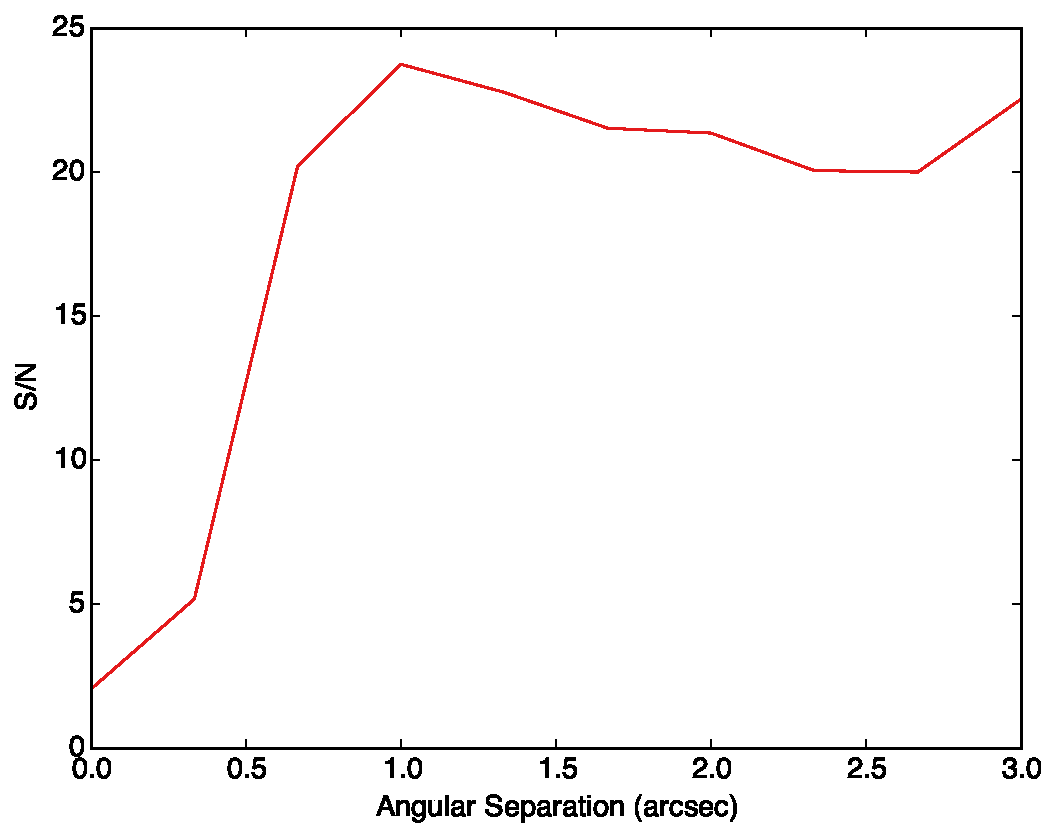
\includegraphics[width=\textwidth]{adi_contrastCurve_amp=2000}
   \caption{Contrast curve for image that is shown in Figure
     \ref{fig:adi_fakeplanet} . The PSF that used as fake planet is
     scaled the same way as in Figure \ref{fig:median_fakeplanet}}
   \label{fig:adi_median_curve}
 \end{figure}

 \subsection{ADI with centering error}
 If $\pm 5$ pixels uncertainties in x and y coordinates are added, the
 performance of ADI reduced significantly. All planets are barely
 seen. Therefore, precisely align images is essential in high contrast
 image processing.
 \begin{figure}
   \centering
   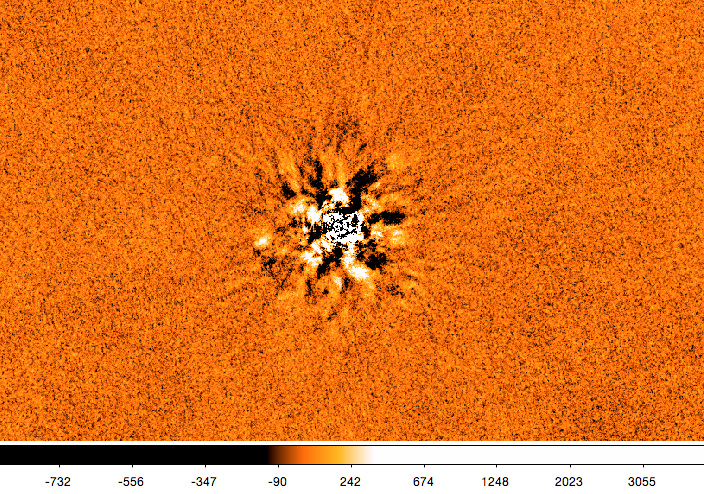
\includegraphics[width=0.48\textwidth]{adi_with_error}
   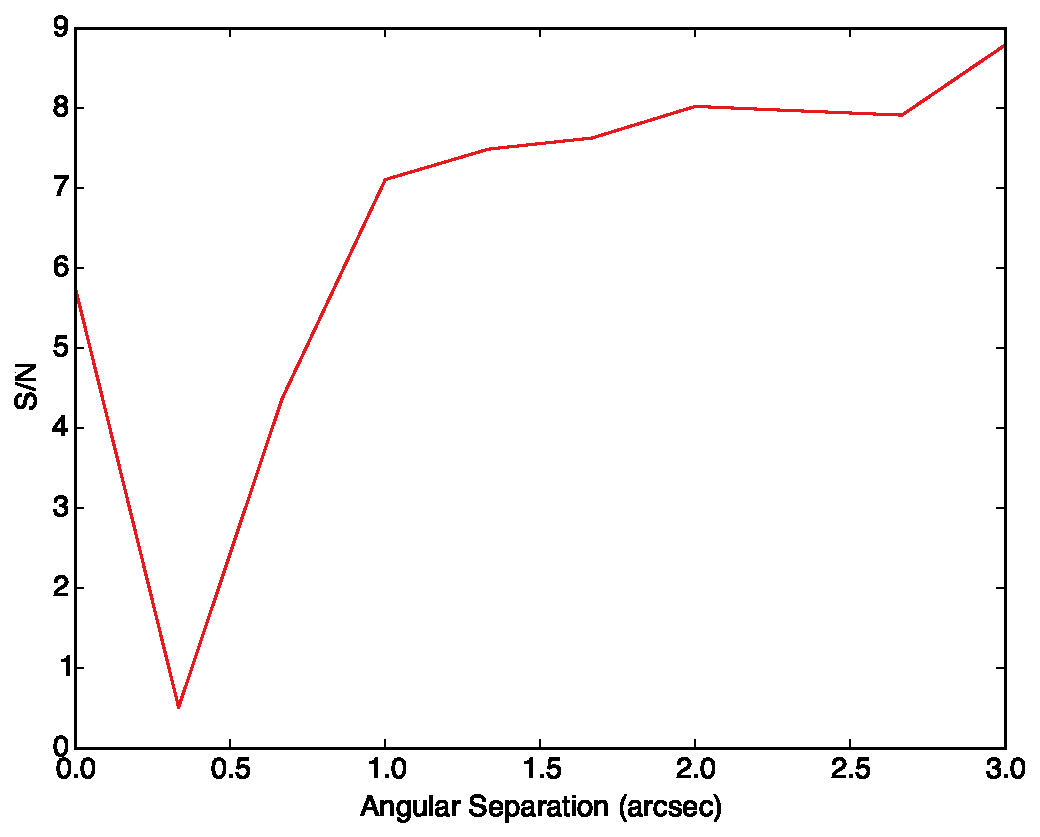
\includegraphics[width=0.48\textwidth]{adiwithErrorCurve}
   \caption{ADI wiht centering error. All planets are barely seen}
   \label{fig:adi_with_error}
 \end{figure}
 
   \section{LOCI}
   \begin{figure}
     \centering
    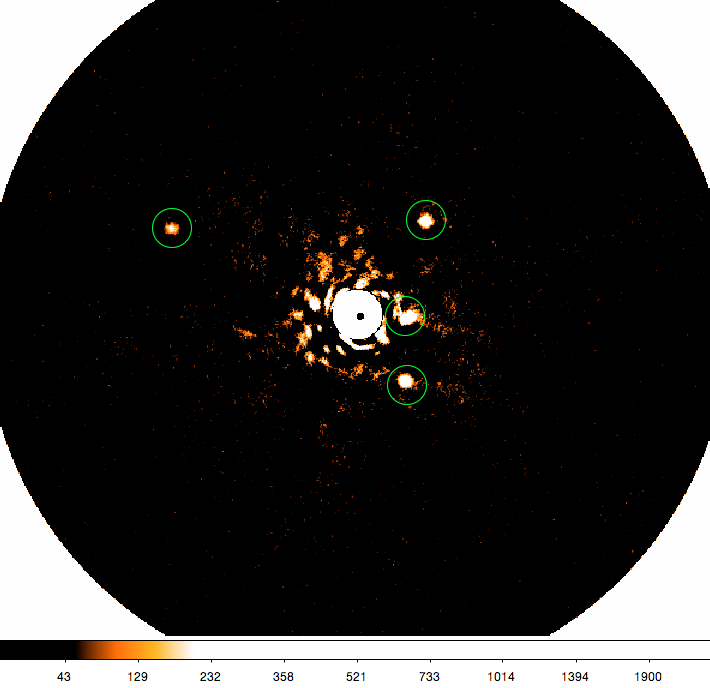
\includegraphics[width=\textwidth]{loci}
     \caption{Image processed by LOCI}
     \label{fig:loci}
   \end{figure}

   \begin{table}[h]
     \centering
          \caption{Star/planet brightness ratio of HR8799 system measured
       from LOCI image}
     \begin{tabular}{|c|c|c|c|c|}
       \hline
       Planet&b&c&d&e\\\hline
       $\Delta$mag&10.71&10.0&9.72&9.02\\\hline
     \end{tabular}
     \label{tab:ratio}
   \end{table}
\end{document}
%%% Local Variables:
%%% mode: latex
%%% TeX-master: t
%%% End:
